\section{Mức độ 5,6 điểm}
\Opensolutionfile{ans}[ans/CD9/Muc_5_6]
\setcounter{dang}{0}
\setcounter{ex}{0}
\begin{dang}
	{Xác định đường tiệm cận thông qua bảng biến thiên, đồ thị}
\end{dang}
\begin{ex}%[2H1Y1-2]
	\immini{
		Hình đa diện trong hình vẽ bên có bao nhiêu mặt?
		\choice
		{$10$}
		{$6$}
		{$12$}
		{\True $11$}
	}{
		\begin{tikzpicture}[line cap=round,line join=round,>=triangle 45,x=1.0cm,y=1.0cm,scale=0.7]
			\draw (0,0)-- (0,1) -- (4,4) -- (6,1) --(6,0)--(5.5,-1)--(3.2,-1.3)--(0,0);
			\draw (0,1) -- (3,0) -- (4,4) --(5,0)--(6,1);
			\draw (3.2,-1.3) -- (3,0) -- (5,0)--(5.5,-1);
			\draw [dashed] (6,1)-- (3,2)-- (0,1) (6,0)--(3,1)--(0,0) (3,1)--(3,2)--(4,4);
		\end{tikzpicture}
	}
	\loigiai{Hình chóp có $5$ mặt tam giác và $5$ mặt tứ giác và một mặt đáy. Vậy có $11$ mặt.}
\end{ex}
\begin{ex}%[2H1Y1-2]
	\immini{Hình đa diện sau có bao nhiêu cạnh?
		\choice
		{$15$}
		{$12$}
		{$20$}
		{\True $16$}}
	{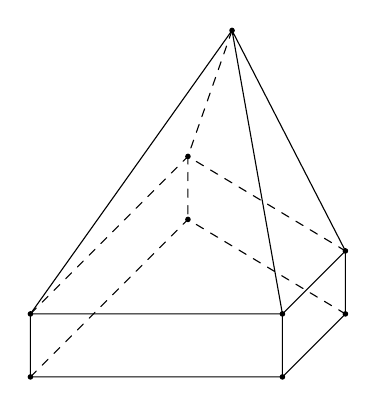
\begin{tikzpicture}[scale=0.8,>=stealth, font=\footnotesize, line join=round, line cap=round]
			\path
			(0,0) coordinate (A)
			(4,0) coordinate (B)
			(5,1) coordinate (C)
			(2.5,2.5) coordinate (D)
			(0,1) coordinate (A')
			(4,1) coordinate (B')
			(5,2) coordinate (C')
			(2.5,3.5) coordinate (D')
			(3.2,5.5) coordinate (S)
			;
			\foreach \d in {A,B,C,D,A',B',C',D',S}
			\draw[fill=black](\d)circle(1pt);
			\draw (A)--(B)--(C)--(C')--(S)--(A')--(B')--(C') (S)--(B') (A)--(A') (B)--(B');
			\draw[dashed] (A)--(D)--(C) (A')--(D')--(C') (S)--(D')--(D);
	\end{tikzpicture}}
\end{ex}

\begin{ex}%[2H1Y1-2]
	Hình chóp ngũ giác có bao nhiêu mặt?
	\choice
	{$7$}
	{\True $6$}
	{$5$}
	{$10$}
	\loigiai{Hình chóp ngũ giác có $5$ mặt bên và $1$ mặt đáy, nên tổng cộng có $6$ mặt.}
\end{ex}
\begin{ex}%[2H1Y1-2]
	Trong một khối đa diện, mệnh đề nào sau đây \textbf{đúng}?
	\choice
	{Hai cạnh bất kỳ có ít nhất một điểm chung}
	{Ba mặt bất kì có ít nhất một đỉnh chung}
	{Hai mặt bất kì có ít nhất một điểm chung}
	{\True Mỗi đỉnh là đỉnh chung của ít nhất ba mặt}
	\loigiai{Ta có tính chất "Mỗi đỉnh là đỉnh chung của ít nhất ba mặt" là tính chất đúng của khối đa diện.}
\end{ex}
\begin{ex}%[2H1Y1-2]
	Trong các mệnh đề sau, mệnh đề nào \textbf{đúng}?
	\choice
	{\True Tồn tại hình đa diện có số đỉnh và số mặt bằng nhau}
	{Số đỉnh và số mặt của một hình đa diện luôn bằng nhau}
	{Tồn tại một hình đa diện có số cạnh và số mặt bằng nhau}
	{Tồn tại một hình đa diện có số cạnh bằng số đỉnh}
	\loigiai{Hình tứ diện có số đỉnh bằng số mặt và bằng $4$.}
\end{ex}
\begin{ex}%[2H1Y1-2]
	Hình nào sau đây \textbf{không} phải là hình đa diện?
	\choice
	{Hình lăng trụ}
	{Hình chóp}
	{Hình lập phương}
	{\True Hình vuông}
	\loigiai{Hình vuông không phải hình đa diện.}
\end{ex}
\begin{ex}%[2H1Y1-2]
	Cho các mệnh đề sau:
	\begin{itemize}
		\item[I.] Số cạnh của một khối đa diện lồi luôn lớn hơn hoặc bằng $6$.
		\item[II.] Số mặt của khối đa diện lồi luôn lớn hơn hoặc bằng $5$.
		\item[III.] Số đỉnh của khối đa diện lồi luôn lớn hơn $4$.
	\end{itemize}
	Trong các mệnh đề trên, những mệnh đề nào là mệnh đề đúng?
	\choice
	{$II$ và $III$}
	{$I$ và $II$}
	{\True Chỉ $I$}
	{Chỉ $II$}
	\loigiai{Mệnh đề II sai vì khối tứ diện là khối đa diện lồi có số mặt nhỏ hơn $5$. \\
		Mệnh đề III sai vì khối tứ diện là khối đa diện lồi có $4$ đỉnh.
	}
\end{ex}
\begin{ex}%[2H1Y1-2]
	Cho khối đa diện đều. Khẳng định nào sau đây là \textbf{sai}?
	\choice
	{Số đỉnh của khối lập phương là $8$}
	{Số mặt của khối tứ diện đều bằng $4$}
	{\True Khối bát diện đều là loại $\{4;3\}$}
	{Số cạnh của khối bát diện đều bằng $12$}
	\loigiai{Khối bát diện đều là loại $\{3;4\}$.}
\end{ex}
\begin{ex}%[2H1Y1-2]
	Có tất cả bao nhiêu khối đa diện đều
	\choice
	{$6$}
	{$7$}
	{\True $5$}
	{$4$}
	\loigiai{Có tất cả $5$ khối đa diện đều là: Khối tứ diện đều, khối lập phương, khối bát diện đều (hay khối tám mặt đều), khối mười hai mặt đều và khối hai mươi mặt đều.}
\end{ex}
\begin{ex}%[2H1Y1-2]%[THPT Phan Đăng Lưu - Huế -2018]
	Số cạnh của hình mười hai mặt đều là
	\choice
	{$20$}
	{\True $30$}
	{$16$}
	{$12$}
	\loigiai{
		Hình mười hai mặt đều có $30$ cạnh.
	}
\end{ex}
\begin{ex}%[2H1Y1-1]%[THPT Chuyên Biên Hòa - Hà Nam - 2018] 
	Hình nào dưới đây không phải là hình đa diện?
	\begin{center}
		\begin{minipage}{4cm}
			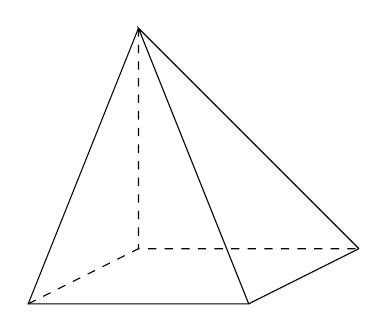
\begin{tikzpicture}[scale=0.7]
				\draw [dashed] (-1,-2)-- (1,-1)-- (5,-1) (1,3)-- (1,-1);
				\draw (5,-1)-- (3,-2)--(1,3)--(5,-1) (3,-2)-- (-1,-2)--(1,3);
			\end{tikzpicture}
			\centering{\textbf{Hình 1}}
		\end{minipage}
		\begin{minipage}{4cm}
			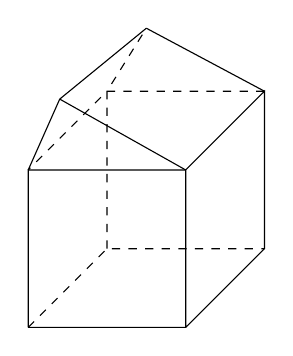
\begin{tikzpicture}[scale=1]
				\draw (0,0)-- (2,0)--(2,2)--(0,2)--(0,0) (2,0)-- (3,1)--(3,3)--(2,2) (1.5,3.8)--(3,3);
				\draw [dashed] (3,3)-- (1,3)--(0,2) (0,0)--(1,1)--(3,1) (1,1)--(1,3)--(1.5,3.8);
				\draw (0,2)--(0.4,2.9)--(1.5,3.8) (0.4,2.9)--(2,2);
			\end{tikzpicture}
			\centering{\textbf{Hình 2}}
		\end{minipage}
		\begin{minipage}{4cm}
			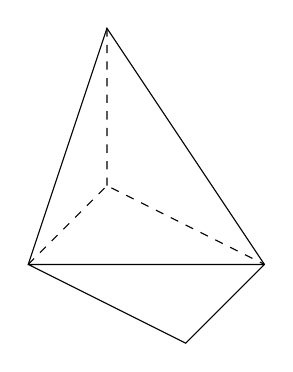
\begin{tikzpicture}
				\draw [dashed] (0,0)-- (1,1)--(3,0) (1,3)--(1,1);
				\draw (0,0)-- (2,-1)--(3,0)--(1,3)--(0,0)--(3,0);
			\end{tikzpicture}\\
			\centering{\textbf{Hình 3}}
		\end{minipage}
		\begin{minipage}{4cm}
			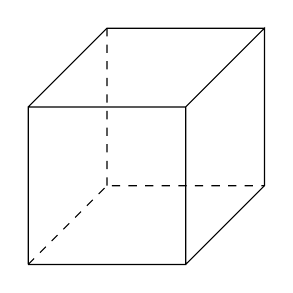
\begin{tikzpicture}[scale=1]
				\draw (0,0)-- (2,0)--(2,2)--(0,2)--(0,0) (2,0)-- (3,1)--(3,3)--(2,2) (3,3)-- (1,3)--(0,2);
				\draw [dashed] (0,0)--(1,1)--(3,1) (1,1)--(1,3);
			\end{tikzpicture}
			\centering{\textbf{Hình 4}}
		\end{minipage}
	\end{center}
	\choice
	{Hình 1}
	{Hình 2}
	{\True Hình 3}
	{Hình 4}
	\loigiai{
		Hình đa diện gồm một số hữu hạn đa giác phẳng thỏa mãn hai điều kiện sau:
		\begin{itemize}
			\item Hai đa giác bất kì hoặc không có điểm chung, hoặc có một đỉnh chung, hoặc có một cạnh chung.
			\item Mỗi cạnh của một đa giác là cạnh chung của đúng hai đa giác.
		\end{itemize}
		Vậy hình 3 có một cạnh là cạnh chung của $3$ mặt nên hình 3 không phải hình đa diện.
	}
\end{ex}

\begin{ex}%[2H1Y2-2]%[THPT Đoàn Thượng - Hải Phòng - 2018]
	Khối đa diện đều loại $\{3; 5\}$ là khối
	\choice
	{\True hai mươi mặt đều}
	{tám mặt đều}
	{lập phương}
	{tứ diện đều}
	\loigiai{
		Khối đa diện đều loại $\{3; 5\}$ là khối hai mươi mặt đều.
	}
\end{ex}
\begin{ex}%[2H1Y1-2]
	\immini{
		Hình vẽ bên có bao nhiêu mặt?
		\choice
		{ $7$}
		{\True $9$}
		{ $4$}
		{ $10$}
	}
	{
		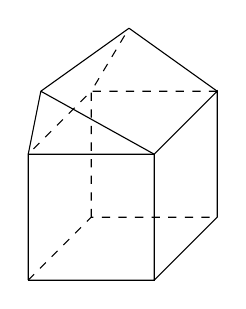
\begin{tikzpicture}[scale=0.8]
			\draw (0,0)-- (2,0)--(2,2)--(0,2)--(0,0) (2,0)-- (3,1)--(3,3)--(2,2) (1.6,4)--(3,3);
			\draw [dashed] (3,3)-- (1,3)--(0,2) (0,0)--(1,1)--(3,1) (1,1)--(1,3)--(1.6,4);
			\draw (0,2)-- (0.2,3)--(1.6,4) (0.2,3)--(2,2);
		\end{tikzpicture}
	}
	\loigiai{
		Hình vẽ đã cho có $9$ mặt.}
\end{ex}

\begin{ex}%[2H1Y2-2]%[THPT Chuyên LHP – 2017]
	Biết $(H)$  là đa diện đều loại $\{3; 5\}$ với số đỉnh và số cạnh lần lượt là $a$ và $b$. Giá trị $a-b$ bằng
	\choice
	{$18$}
	{$-8$}
	{\True $-18$}
	{$10$}
	\loigiai{
		Khối đa diện đều loại $\{3; 5\}$ có số đỉnh $a=12$ và số cạnh $b=30$.\\
		Vậy $a-b=-18$.
	}
\end{ex}
\begin{ex}%[2H1Y1-1]%[THPT Can Lộc - Hà Tĩnh - 2018]
	Gọi $ n$ là số hình đa diện trong bốn hình bên dưới. Tìm $ n$.
	\begin{center}
		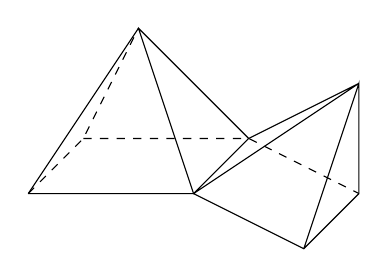
\begin{tikzpicture}[scale=0.7]
			\draw [dashed] (0,-1)-- (1,0)-- (2,2) (1,0)-- (4,0)-- (6,-1);
			\draw (0,-1)-- (2,2)-- (3,-1)-- (4,0)-- (2,2) (0,-1)-- (3,-1) (3,-1)-- (5,-2)-- (6,-1)-- (6,1)-- (5,-2) (3,-1)-- (6,1)-- (4,0);
		\end{tikzpicture}~~
		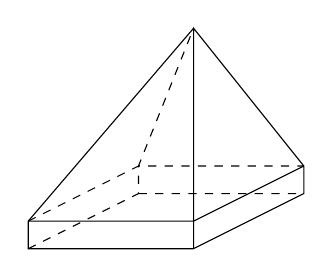
\begin{tikzpicture}[scale=0.7]
			\draw [dashed] (0,0)-- (2,1)-- (2,1.5)-- (3,4) (0,0.5)-- (2,1.5)-- (5,1.5) (2,1)-- (5,1);
			\draw (3,4)-- (0,0.5)-- (0,0)-- (3,0)-- (5,1)-- (5,1.5)-- (3,4)--(3,0) (0,0.5)-- (3,0.5)-- (5,1.5);
		\end{tikzpicture}~~
		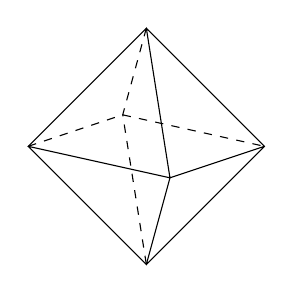
\begin{tikzpicture}[scale=1]
			\draw(3,0)--(1.8,-0.4)--(0,0)--(1.5,1.5)--(1.8,-0.4)--(1.5,-1.5)--(0,0) (1.5,-1.5)--(3,0)--(1.5,1.5);
			\draw[dashed] (0,0)--(1.2,0.4) --(3,0) (1.5,1.5)--(1.2,0.4)--(1.5,-1.5);
		\end{tikzpicture}~~
		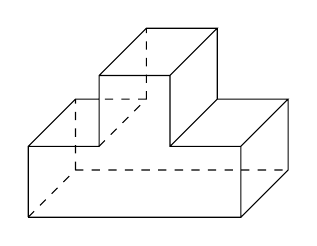
\begin{tikzpicture}[scale=0.6]
			\draw [dashed] (0,0)-- (1,1)-- (5.5,1) (1,1)-- (1,2.5) (1.5,1.5)-- (2.5,2.5)-- (2.5,4) (2.5,2.5)-- (1.5,2.5);
			\draw (0,0)-- (0,1.5)-- (1.5,1.5)-- (1.5,3)-- (2.5,4)-- (4,4)-- (3,3)-- (1.5,3) (3,3)--(3,1.5)-- (4.5,1.5)-- (5.5,2.5)-- (4,2.5)-- (4,4) (4,2.5)-- (3,1.5) (1.5,2.5)-- (1,2.5)-- (0,1.5) (0,0)-- (4.5,0)-- (4.5,1.5) (4.5,0)--(5.5,1)-- (5.5,2.5);
		\end{tikzpicture}
	\end{center}
	\choice
	{\True $n=3$}
	{$n=1$}
	{$n=2$}
	{$n=4$}
	\loigiai{
		\immini{
			Có $3$ hình đa diện trong số các hình đã cho.\\
			Hình bên không phải đa diện vì có một cạnh là cạnh chung của $4$ mặt.
		}
		{
			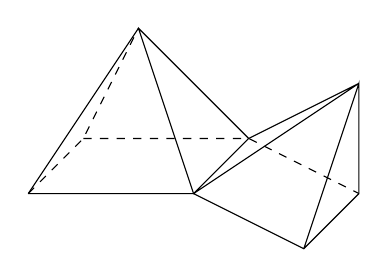
\begin{tikzpicture}[scale=0.7]
				\draw [dashed] (0,-1)-- (1,0)-- (2,2) (1,0)-- (4,0)-- (6,-1);
				\draw (0,-1)-- (2,2)-- (3,-1)-- (4,0)-- (2,2) (0,-1)-- (3,-1) (3,-1)-- (5,-2)-- (6,-1)-- (6,1)-- (5,-2) (3,-1)-- (6,1)-- (4,0);
			\end{tikzpicture}
		}
	}
\end{ex}
\begin{ex}%[2H1B2-2]%[SGD Bình Dương - 2018]
	Khối đa diện đều loại $\{4;3\}$ là
	\choice
	{Khối tứ diện đều}
	{\True Khối lập phương}
	{Khối bát diện đều}
	{Khối hộp chữ nhật}
	\loigiai{
		Theo định nghĩa, khối đa diện đều loại $\{4;3\}$ là khối có:
		\begin{itemize}
			\item Mỗi mặt là $1$ đa giác đều có $4$ cạnh (hình vuông).
			\item Mỗi đỉnh là đỉnh chun của đúng $3$ mặt.
		\end{itemize}
		Vậy nó là khối lập phương.
		\begin{center}
			Bảng tóm tắt về năm loại khối đa diện đều\\
			\begin{tabular}{|c|c|c|c|c|}
				\hline 
				Loại & Tên gọi & Số đỉnh & Số cạnh & Số mặt \\
				\hline 
				$\{3;3\}$ & Tứ diện đều & $4$ & $6$ & $4$\\
				\hline 
				$\{4;3\}$ & Lập phương & $8$ & $12$ & $6$\\
				\hline 
				$\{3;4\}$ & Bát diện đều & $6$ & $12$ & $6$\\
				\hline 
				$\{5;3\}$ & Mười hai mặt đều & $20$ & $30$ & $12$\\
				\hline 
				$\{3;5\}$ & Hai mươi mặt đều & $12$ & $30$ & $20$\\
				\hline
			\end{tabular}
		\end{center}
	}
\end{ex}

%Câu 17
\begin{ex}%[2H1Y2-2]%[Chuyên Tuyên Quang  - 2017]
	Khối đa diện đều nào sau đây có mặt {\bf không phải} là tam giác đều?
	\choice
	{Bát diện đều}
	{Tứ diện dều}
	{\True Mười hai mặt đều}
	{Hai mươi mặt đều}
	\loigiai{
		\immini{
			Hình khối $12$ mặt đều có mỗi mặt là một ngũ giác đều.
		}
		{
			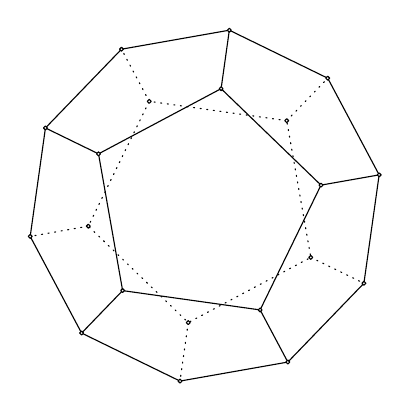
\begin{tikzpicture}[>=stealth,line join=round,line cap=round,font=\footnotesize,scale=0.5]
				\def\r{3}
				\def\gA{10}
				\path
				(\gA:\r) coordinate (A_1)
				(\gA+72:\r) coordinate (A_2)
				(\gA+144:\r) coordinate (A_3)
				(\gA+216:\r) coordinate (A_4)
				(\gA+288:\r) coordinate (A_5)
				(\gA+36:\r) coordinate (B_1)
				(\gA+108:\r) coordinate (B_2)
				(\gA+180:\r) coordinate (B_3)
				(\gA+252:\r) coordinate (B_4)
				(\gA+324:\r) coordinate (B_5)
				\foreach \i in {1,...,10}{(\gA+\i *36-36:1.5*\r) coordinate (C_\i)}
				;
				\draw[dotted]
				(B_1)--(B_2) --(B_3)--(B_4)--(B_5)--cycle
				(B_1)--(C_2) (B_2)--(C_4) (B_3)--(C_6) (B_4)--(C_8) (B_5)--(C_10)
				;
				\draw
				(A_1)--(A_2)--(A_3)--(A_4)--(A_5)--cycle
				(A_1)--(C_1) (A_2)--(C_3) (A_3)--(C_5) (A_4)--(C_7) (A_5)--(C_9)
				(C_1)--(C_2)--(C_3)--(C_4)--(C_5)--(C_6)--(C_7)--(C_8) --(C_9)--(C_10)--cycle
				;
				\foreach \x in {A_1,A_2,A_3,A_4,A_5,B_1,B_2,B_3,B_4,B_5,C_1,C_2,C_3, C_4,C_5,C_6,C_7, C_8,C_9,C_10} \draw[fill=white] (\x) circle (.05);
			\end{tikzpicture}
		}
	}
\end{ex}

%Câu 18
\begin{ex}%[2H1Y2-1]%[THPT Đô Lương 4 - Nghệ An -2018]
	Số hình đa diện lồi trong các hình dưới đây là
	\begin{center}
		\begin{tikzpicture}[scale=0.5]
			\path
			(0,0) coordinate (A1)
			(4,0) coordinate (A2)
			(1.75,1.15) coordinate (A4)
			($(A2)+(A4)-(A1)$)coordinate (A3)
			($(A1)+(1.2,2.5)$)coordinate (B1)
			($(A1)+(3.5,2.5)$)coordinate (B2)
			($(A1)+(2.5,3)$)coordinate (B4)
			($(B2)+(B4)-(B1)$)coordinate (B3)
			($(B1)+(-.25,.75)$)coordinate (C1)
			($(B2)+(.3,.5)$)coordinate (C2)
			($(B3)+(.3,.5)$)coordinate (C3)
			($(B4)+(-.25,.75)$)coordinate (C4)
			;
			\draw[dashed]
			(A1)--(A4)--(A3)
			(B1)--(B4)--(B3) (A4)--(B4) (B4)--(C4)
			;
			\draw 
			(A1)--(A2)--(A3) (A1)--(B1)--(B2)--(B3) (A2)--(B2) (A3)--(B3)
			(B1)--(C1)--(C2)--(C3)--(C4)--(C1) (B2)--(C2) (B3)--(C3)
			;
		\end{tikzpicture}
		\hspace*{1.25cm}
		\begin{tikzpicture}[scale=0.6]
			\path
			(0,0) coordinate (A1)
			(3,-.75) coordinate (A2)
			(4,0) coordinate (A3)
			($(A1)+(A3)-(A2)$)coordinate (A4)
			($(A2)+(.5,1.5)$)coordinate (B1)
			($(A1)+(B1)-(A2)$)coordinate (B2)
			($(A3)+(.3,1)$)coordinate (A5)
			($(A5)+(-.5,1)$)coordinate (B3)
			(intersection of A4--B3 and B1--B2) coordinate (E)
			;
			\draw[dashed]
			(A1)--(A4)--(A3) (B2)--(A4)--(A5) (A4)--(E)
			;
			\draw 
			(A1)--(A2)--(A3) (A2)--(B1)--(A3) (A1)--(B2)--(B1) (E)--(B3)
			(A3)--(A5)--(B3)--(A3)
			;
		\end{tikzpicture}
		\hspace*{1.25cm}
		\begin{tikzpicture}[scale=0.5]
			\path
			(0,0) coordinate (A1)
			(4,0) coordinate (A2)
			(1.75,1.15) coordinate (A4)
			($(A2)+(A4)-(A1)$)coordinate (A3)
			($(A1)+(2,4)$)coordinate (S)
			;
			\draw[dashed]
			(A4)--(A3)
			;
			\draw 
			(S)--(A1)--(A4)--(A2)--(A3)--(S)--(A4) (S)--(A2)
			;
		\end{tikzpicture}
		\hspace*{1.25cm}
		\begin{tikzpicture}[scale=0.6]
			\path
			(0,0) coordinate (A1)
			(2,0) coordinate (A2)
			(-1,1) coordinate (A4)
			($(A2)+(A4)-(A1)$)coordinate (A3)
			($(A1)+(0,1.5)$)coordinate (B1)
			($(A2)+(0,1.5)$)coordinate (B2)
			($(A3)+(0,1.5)$)coordinate (B3)
			($(A4)+(0,1.5)$)coordinate (B4)
			($(B1)!.3!(B2)$)coordinate (B5)
			($(B5)+(0,.75)$) coordinate (C1)
			($(A4)+(C1)-(A1)$) coordinate (C2)
			;
			\draw[dashed]
			(A4)--(A3)--(A2)
			(B3)--(A3) (B3)--(B4)
			;
			\draw 
			(A4)--(A1)--(A2) (B4)--(B1)--(B2)--(B3) (B1)--(A1) (B2)--(A2) (B4)--(A4) (B1)--(C1)--(B2) (C1)--(C2)--(B4) (C2)--(B3)
			;
		\end{tikzpicture}
	\end{center}
	\choice
	{$0$}
	{\True $1$}
	{$2$}
	{$3$}
	\loigiai{
		\immini 
		{Trong các hình đã cho, chỉ có hình bên là đa diện lồi vì thỏa mãn nếu lấy bất kì hai điểm nào thì đoạn thẳng nối hai điểm đó nằm trong khối đa diện.
			Vậy chỉ có $1$ đa diện lồi.
		}
		{
			\begin{tikzpicture}[scale=0.6]
				\path
				(0,0) coordinate (A1)
				(2,0) coordinate (A2)
				(-1,1) coordinate (A4)
				($(A2)+(A4)-(A1)$)coordinate (A3)
				($(A1)+(0,1.5)$)coordinate (B1)
				($(A2)+(0,1.5)$)coordinate (B2)
				($(A3)+(0,1.5)$)coordinate (B3)
				($(A4)+(0,1.5)$)coordinate (B4)
				($(B1)!.3!(B2)$)coordinate (B5)
				($(B5)+(0,.75)$) coordinate (C1)
				($(A4)+(C1)-(A1)$) coordinate (C2)
				;
				\draw[dashed]
				(A4)--(A3)--(A2)
				(B3)--(A3) (B3)--(B4)
				;
				\draw 
				(A4)--(A1)--(A2) (B4)--(B1)--(B2)--(B3) (B1)--(A1) (B2)--(A2) (B4)--(A4) (B1)--(C1)--(B2) (C1)--(C2)--(B4) (C2)--(B3)
				;
			\end{tikzpicture}
		}		
	}
\end{ex}

%Câu 19
\begin{ex}%[2H1B2-2]%[THPT Thanh Miện - Hải Dương - 2018]
	Cho khối đa diện đều loại $\{3;4\}$. Tổng các góc phẳng tại $1$ đỉnh của khối đa diện bằng
	\choice
	{$324^\circ$}
	{$360^\circ$}
	{$180^\circ$}
	{\True $240^\circ$}
	\loigiai{
		Khối đa diện đều loại $\{3;4\}$ là khôi bát diện đều, mỗi mặt là một tam giác đều và mỗi đỉnh là đỉnh chung của $4$ mặt nên tổng các góc tại $1$ đỉnh là $240^\circ$.
	}
\end{ex}

%Câu 20
\begin{ex}%[2H1Y1-1]%[Chuyên Hưng Yên - 2017]
	Hình nào dưới đây {\bf không phải} là một khối đa diện?
	\choice
	{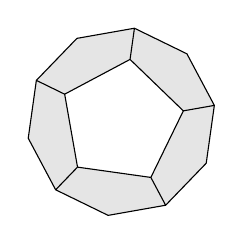
\begin{tikzpicture}[>=stealth,line join=round,line cap=round,font=\footnotesize,scale=0.8]
			\def\r{1}
			\def\gA{10}
			\path
			(\gA:\r) coordinate (A_1)
			(\gA+72:\r) coordinate (A_2)
			(\gA+144:\r) coordinate (A_3)
			(\gA+216:\r) coordinate (A_4)
			(\gA+288:\r) coordinate (A_5)
			(\gA+36:\r) coordinate (B_1)
			(\gA+108:\r) coordinate (B_2)
			(\gA+180:\r) coordinate (B_3)
			(\gA+252:\r) coordinate (B_4)
			(\gA+324:\r) coordinate (B_5)
			\foreach \i in {1,...,10}{(\gA+\i *36-36:1.5*\r) coordinate (C_\i)}
			;
			% \draw[dotted]
			% (B_1)--(B_2) --(B_3)--(B_4)--(B_5)--cycle
			% (B_1)--(C_2) (B_2)--(C_4) (B_3)--(C_6) (B_4)--(C_8) (B_5)--(C_10)
			% ;
			\foreach \a/\b/\c/\d/\e in 
			{
				A_3/C_5/C_4/C_3/A_2,
				A_2/C_3/C_2/C_1/A_1,
				A_1/C_1/C_10/C_9/A_5,
				A_5/C_9/C_8/C_7/A_4,
				A_4/C_7/C_6/C_5/A_3,
				A_3/C_5/C_4/C_3/A_2}
			{\fill[black!10] (\a)--(\b)--(\c)--(\d)--(\e)--cycle;}
			\draw
			(A_1)--(A_2)--(A_3)--(A_4)--(A_5)--cycle
			(A_1)--(C_1) (A_2)--(C_3) (A_3)--(C_5) (A_4)--(C_7) (A_5)--(C_9)
			(C_1)--(C_2)--(C_3)--(C_4)--(C_5)--(C_6)--(C_7)--(C_8) --(C_9)--(C_10)--cycle
			;
			% \fill[gray,opacity=0.7]
			% (A_1)--(B_1)--(B_2)--(A_2)--cycle
			% ;
			% \foreach \x in {A_1,A_2,A_3,A_4,A_5,B_1,B_2,B_3,B_4,B_5,C_1,C_2,C_3, C_4,C_5,C_6,C_7, C_8,C_9,C_10} \draw[fill=white] (\x) circle (.05)node{$\x$};
		\end{tikzpicture}
	}
	{
		\begin{tikzpicture}[>=stealth,line join=round,line cap=round,font=\footnotesize,scale=0.6]
			\def\h{3.5}
			\def\ac{4}
			\def\xb{1}
			\def\yb{-1.25}
			\coordinate (A) at (0,0);
			\coordinate (B) at (\xb,\yb);
			\coordinate (C) at (\ac,0);
			\coordinate (O) at ($($(B)!0.5!(C)$)!1/3!(A)$);
			\coordinate (S) at ($(O)+(0,\h)$);
			\fill[black!10] 
			(S)--(A)--(B)--cycle;
			\fill[black!10]
			(S)--(B)--(C)--cycle;
			\draw 
			(S)--(A)--(B)--(C)--cycle
			(S)--(B);
			% \foreach \point in {A,B,C,S,O}
			% 	\fill (\point) circle (1pt);
		\end{tikzpicture}
	}
	{\begin{tikzpicture}[>=stealth,line join=round,line cap=round,font=\footnotesize,scale=0.8]
			\path (0,0) coordinate (A) ++(90:2.4) coordinate (B) ++(180:.7) coordinate (C) 
			++(90:.4) coordinate (D) ++(0:2.1) coordinate (E) ++(-90:.4) coordinate (F) 
			++(180:.7) coordinate (G) ++(-90:2.4) coordinate (H) ($(D)+(45:.4)$) coordinate (D')
			++(0:2.1) coordinate (E') ++(-90:.4) coordinate (F')
			++(180:.7) coordinate (G') ++(-90:2.2) coordinate (H')
			(intersection of F--G and G'--H')coordinate (I);
			\fill[black!10](D)--(D')--(E')--(F')--(F)--(E)--cycle;
			\fill[black!10](H)--(G)--(I)--(H')--cycle;
			\draw (A)--(B)--(C)--(D)--(E)--(F)--(G)--(H)--cycle
			(D)--(D')--(E')--(F')--(F) (I)--(H')--(H) (E)--(E');
		\end{tikzpicture}
	}
	{\True \begin{tikzpicture}[line join=round,line width=.6pt,scale=0.7]
			\path
			(0,0) coordinate (A) ++(30:2.1) coordinate (B) ++(0:2.5) coordinate (C) ++(-150:2.1) coordinate (D)
			(0,1.4) coordinate (A') ++(30:2.1) coordinate (B') ++(0:2.5) coordinate (C') ++(-150:2.1) coordinate (D')
			($(B')!.5!(D')$) coordinate (S) ++(160:1.8)coordinate (A'')
			++(30:1.6)coordinate (B'') ++(0:1.8)coordinate (C'') ++(-150:1.6)coordinate (D'')
			(intersection of A'--B' and S--A'')coordinate (I1) (intersection of B'--C' and S--C'')coordinate (I2);
			\fill[black!10](A)--(A')--(D')--(C')--(C)--(D)--cycle;
			\fill[black!10](A'')--(S)--(C'')--(D'')--cycle;
			\draw (C')--(C)--(D)--(A)--(A')--(I1) (I2)--(C')--(D')--(A') (D)--(D')
			(A'')--(D'')--(S)--(A'')--(B'')--(C'')--(S) (C'')--(D'');
	\end{tikzpicture}}
	\loigiai{
		\immini{
			Hình bên không phải là khối đa diện
		}
		{
			\begin{tikzpicture}[line join=round,line width=.6pt,scale=0.7]
				\path
				(0,0) coordinate (A) ++(30:2.1) coordinate (B) ++(0:2.5) coordinate (C) ++(-150:2.1) coordinate (D)
				(0,1.4) coordinate (A') ++(30:2.1) coordinate (B') ++(0:2.5) coordinate (C') ++(-150:2.1) coordinate (D')
				($(B')!.5!(D')$) coordinate (S) ++(160:1.8)coordinate (A'')
				++(30:1.6)coordinate (B'') ++(0:1.8)coordinate (C'') ++(-150:1.6)coordinate (D'')
				(intersection of A'--B' and S--A'')coordinate (I1) (intersection of B'--C' and S--C'')coordinate (I2);
				\fill[black!10](A)--(A')--(D')--(C')--(C)--(D)--cycle;
				\fill[black!10](A'')--(S)--(C'')--(D'')--cycle;
				\draw (C')--(C)--(D)--(A)--(A')--(I1) (I2)--(C')--(D')--(A') (D)--(D')
				(A'')--(D'')--(S)--(A'')--(B'')--(C'')--(S) (C'')--(D'');
			\end{tikzpicture}
		}
	}
\end{ex}

%Câu 21
\begin{ex}%[2H1Y1-1]%[THPT Xuân Trường - Nam Định - 2018]
	Hình nào dưới đây {\bf không phải} là hình đa diện?
	\choice
	{\True 
		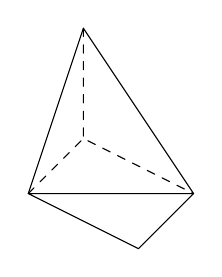
\begin{tikzpicture}[>=stealth,line join=round,line cap=round,font=\footnotesize,scale=0.7]
			\draw [dashed] (0,0)-- (1,1)--(3,0) (1,3)--(1,1);
			\draw (0,0)-- (2,-1)--(3,0)--(1,3)--(0,0)--(3,0);
	\end{tikzpicture}}
	{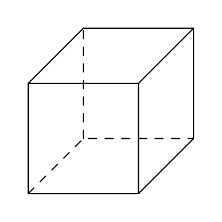
\begin{tikzpicture}[>=stealth,line join=round,line cap=round,font=\footnotesize,scale=0.7]
			\draw (0,0)-- (2,0)--(2,2)--(0,2)--(0,0) (2,0)-- (3,1)--(3,3)--(2,2) (3,3)-- (1,3)--(0,2);
			\draw [dashed] (0,0)--(1,1)--(3,1) (1,1)--(1,3);
	\end{tikzpicture}}
	{
		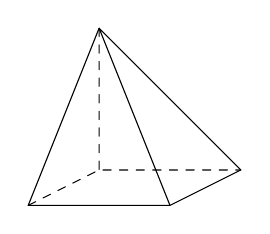
\begin{tikzpicture}[>=stealth,line join=round,line cap=round,font=\footnotesize,scale=0.45]
			\draw [dashed] (-1,-2)-- (1,-1)-- (5,-1) (1,3)-- (1,-1);
			\draw (5,-1)-- (3,-2)--(1,3)--(5,-1) (3,-2)-- (-1,-2)--(1,3);
		\end{tikzpicture}
	}
	{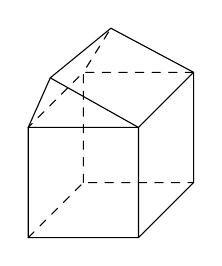
\begin{tikzpicture}[>=stealth,line join=round,line cap=round,font=\footnotesize,scale=0.7]
			\draw (0,0)-- (2,0)--(2,2)--(0,2)--(0,0) (2,0)-- (3,1)--(3,3)--(2,2) (1.5,3.8)--(3,3);
			\draw [dashed] (3,3)-- (1,3)--(0,2) (0,0)--(1,1)--(3,1) (1,1)--(1,3)--(1.5,3.8);
			\draw (0,2)--(0.4,2.9)--(1.5,3.8) (0.4,2.9)--(2,2);
	\end{tikzpicture}}
	\loigiai{
		\immini
		{
			Hình bên không phải là hình đa diện.
		}
		{
			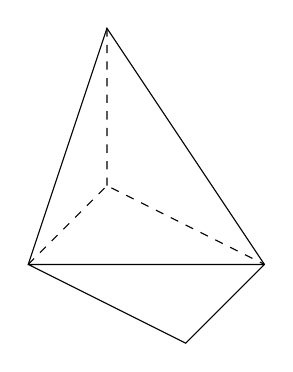
\begin{tikzpicture}
				\draw [dashed] (0,0)-- (1,1)--(3,0) (1,3)--(1,1);
				\draw (0,0)-- (2,-1)--(3,0)--(1,3)--(0,0)--(3,0);
			\end{tikzpicture}
		}
	}
\end{ex}

%Câu 22
\begin{ex}%[2H1B2-2]%[THPT Nguyễn Thị Minh Khai - Hà Tĩnh 2018]
	Khối đa diện $12$ mặt đều có số đỉnh và số cạnh lần lượt là
	\choice
	{$30$ và $20$}
	{$12$ và $20$}
	{\True $20$ và $30$}
	{$12$ và $30$}
	\loigiai{
		\immini{
			Hình khối đa diện $12$ mặt đều có số đỉnh là $20$ và số cạnh là $30$.
		}
		{
			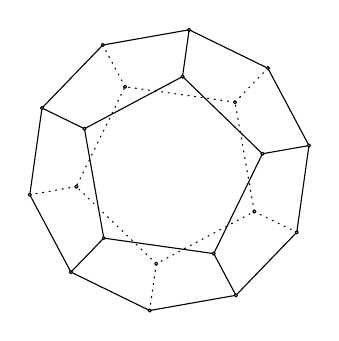
\begin{tikzpicture}[>=stealth,line join=round,line cap=round,font=\footnotesize,scale=0.4]
				\def\r{3}
				\def\gA{10}
				\path
				(\gA:\r) coordinate (A_1)
				(\gA+72:\r) coordinate (A_2)
				(\gA+144:\r) coordinate (A_3)
				(\gA+216:\r) coordinate (A_4)
				(\gA+288:\r) coordinate (A_5)
				(\gA+36:\r) coordinate (B_1)
				(\gA+108:\r) coordinate (B_2)
				(\gA+180:\r) coordinate (B_3)
				(\gA+252:\r) coordinate (B_4)
				(\gA+324:\r) coordinate (B_5)
				\foreach \i in {1,...,10}{(\gA+\i *36-36:1.5*\r) coordinate (C_\i)}
				;
				\draw[dotted]
				(B_1)--(B_2) --(B_3)--(B_4)--(B_5)--cycle
				(B_1)--(C_2) (B_2)--(C_4) (B_3)--(C_6) (B_4)--(C_8) (B_5)--(C_10)
				;
				\draw
				(A_1)--(A_2)--(A_3)--(A_4)--(A_5)--cycle
				(A_1)--(C_1) (A_2)--(C_3) (A_3)--(C_5) (A_4)--(C_7) (A_5)--(C_9)
				(C_1)--(C_2)--(C_3)--(C_4)--(C_5)--(C_6)--(C_7)--(C_8) --(C_9)--(C_10)--cycle
				;
				\foreach \x in {A_1,A_2,A_3,A_4,A_5,B_1,B_2,B_3,B_4,B_5,C_1,C_2,C_3, C_4,C_5,C_6,C_7, C_8,C_9,C_10} \draw[fill=white] (\x) circle (.05);
			\end{tikzpicture}
		}
	}
\end{ex}

%Câu 23
\begin{ex}%[2H1B2-2]%[THPT Lê Quý Đôn - Hải Phòng - 2018]
	Khối hai mươi mặt đều thuộc loại nào sau đây?
	\choice
	{$\{3;4\}$}
	{$\{4;3\}$}
	{\True $\{3;5\}$}
	{$\{5;3\}$}
	\loigiai{
		\immini{
			Khối hai mươi mặt đều có các mặt là tam giác đều và mỗi đỉnh là đỉnh chung của $5$ mặt nên thuộc loại $\{3;5\}$.
		}
		{
			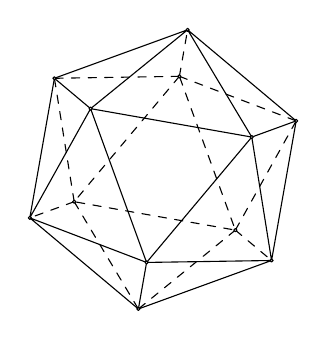
\begin{tikzpicture}[>=stealth,line join=round,line cap=round,font=\footnotesize,scale=0.4]	
				\def\r{3}
				\def\gA{20}
				\path
				(\gA:\r) coordinate (A_1)
				(\gA+120:\r) coordinate (A_2)
				(\gA+240:\r) coordinate (A_3)
				(\gA+60:\r) coordinate (B_1)
				(\gA+180:\r) coordinate (B_2)
				(\gA+300:\r) coordinate (B_3)
				\foreach \i in {1,...,6}{(\gA+\i *60-60:1.5*\r) coordinate (C_\i)}
				;
				\draw[dashed] 
				(B_1)--(B_2)--(B_3)--cycle
				(B_1)--(C_1) (B_1)--(C_2) (B_1)--(C_3)
				(B_2)--(C_3) (B_2)--(C_4) (B_2)--(C_5)
				(B_3)--(C_5) (B_3)--(C_6) (B_3)--(C_1)
				;
				\draw
				(A_1)--(A_2)--(A_3)--cycle
				(A_1)--(C_6) (A_1)--(C_1) (A_1)--(C_2)
				(A_2)--(C_2) (A_2)--(C_3) (A_2)--(C_4)
				(A_3)--(C_4) (A_3)--(C_5) (A_3)--(C_6)
				(C_1)--(C_2) --(C_3)--(C_4)--(C_5)--(C_6)--cycle
				;
				\foreach \x in {A_1,A_2,A_3,B_1,B_2,B_3,C_1,C_2,C_3,C_4,C_5,C_6} \draw[fill=white] (\x) circle (.05);
			\end{tikzpicture}
		}
	}
\end{ex}
\begin{ex}%[2H1Y2-2]
	Khối đa diện có mười hai mặt đều có số đỉnh, số cạnh, số mặt lần lượt là
	\choice
	{$30, 20, 12$}
	{$20, 12, 30$}
	{$12, 30, 20$}
	{\True $20, 30, 12$}
	\loigiai{Khối mười hai mặt đều có $20$ đỉnh, $30$ cạnh và $12$ mặt}
\end{ex}
\begin{ex}%[2H1Y2-1]
	Trong các hình dưới đây, hình nào không phải là đa diện lồi?
	\begin{center}
		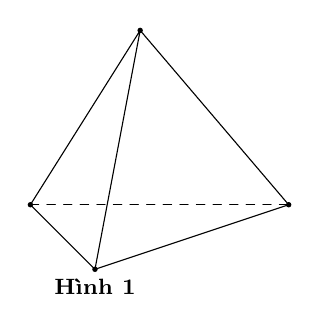
\begin{tikzpicture}[>=stealth,line join=round,line cap=round,font=\footnotesize,scale=.82]
			\coordinate (A) at (0,0);
			\coordinate (B) at (1,-1);
			\coordinate (C) at (4,0);
			\coordinate (S) at (1.7,2.7);
			\draw (A)--(B)--(C)--(S)--cycle (S)--(B);
			\draw[dashed] (A)--(C);
			\fill (A)circle(1.2pt) (B)circle(1.2pt) (C)circle(1.2pt) (S)circle(1.2pt);
			\path(1,-1)node[below]{\textbf{Hình 1}};
		\end{tikzpicture}\hspace{1cm}
		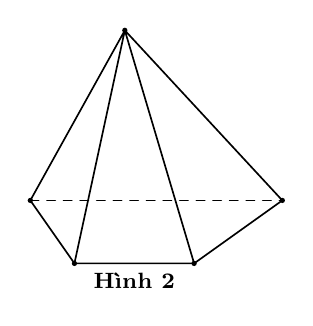
\begin{tikzpicture}[line join=round,line cap=round,line width=.6pt,font=\footnotesize,scale=.8]
			\coordinate (A) at (0,0);
			\coordinate (B) at (.7,-1);
			\coordinate(C) at (2.6,-1);
			\coordinate (D) at (4,0);
			\coordinate (S) at (1.5,2.7);
			\draw (A)--(B)--(C)--(D)--(S)--cycle (B)--(S)--(C);
			\draw[dashed] (A)--(D);
			\path (B)--(C) node[below,midway,sloped]{\textbf{Hình 2}};
			\fill (A)circle(1.2pt) (B)circle(1.2pt) (C)circle(1.2pt) (D)circle(1.2pt) (S)circle(1.2pt);
		\end{tikzpicture}\hspace{1cm}
		\begin{tikzpicture}[line join=round,line cap=round,line width=.6pt,font=\footnotesize,scale=.8]
			\coordinate (A) at (0,0);
			\coordinate (B) at (1,-1);
			\coordinate (C) at (3.5,0);
			\coordinate (A1) at ($(A)+(90:2.7)$);
			\coordinate (B1) at ($(B)-(A)+(A1)$);
			\coordinate (C1) at ($(C)-(A)+(A1)$);
			\draw (A1)--(A)--(B)--(C)--(C1)--(A1)--(B1)--(C1) (B)--(B1);
			\draw[dashed] (A)--(C);
			\fill (A)circle(1.2pt) (B)circle(1.2pt) (C)circle(1.2pt) (A1)circle(1.2pt) (B1)circle(1.2pt) (C1)circle(1.2pt);
			\path (B) node[below]{\textbf{Hình 3}};
		\end{tikzpicture}\hspace{1cm}
		\begin{tikzpicture}[>=stealth,line join=round,line cap=round,font=\footnotesize,scale=.8]
			\def\a{4}
			\path(0,0)coordinate(A)--++(0:\a)coordinate(B)--++(-130:0.4*\a)coordinate(C)--++(-180:0.5*\a)coordinate(D)--++(40:.3*\a)coordinate(E);
			\draw[dashed](A)--(B)(D)--(E)--($ (E)!1/3!(A) $)coordinate(F);
			\draw(B)--(C)--(D)--($ (D)!4.2!(F) $)coordinate(S)--(A)--(F)(C)--(S)--(B);
			\draw[dashed](S)--(E);
			\foreach \x in {A,B,C,D,E,S} \draw[fill=black] (\x) circle (1.1pt);
			\path (C)--(D) node[below,midway,sloped]{\textbf{Hình 4}};
		\end{tikzpicture}
	\end{center}
	\choice
	{\True Hình (IV)}
	{Hình (III)}
	{Hình (II)}
	{Hình (I)}
	\loigiai{Hình IV không phải đa diện lồi}
\end{ex}
\begin{ex}%[2H1Y1-2]
	\immini{Hình đa diện bên có bao nhiêu mặt?
		\choice
		{$7$}
		{$11$}
		{$12$}
		{\True $10$}}
	{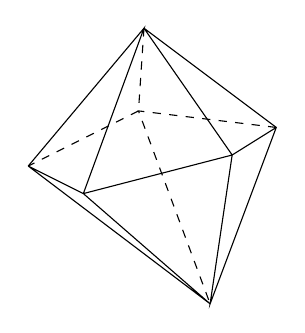
\begin{tikzpicture}[scale=0.7]
			\path
			(0,0) coordinate (A)
			(1,-0.5) coordinate (B)
			(2,1) coordinate (C)
			(2.1,2.5) coordinate (D)
			(3.3,-2.5) coordinate (E)
			(3.7,0.2) coordinate (F)
			(4.5,0.7) coordinate (G)
			;
			\draw (B)--(E)--(A)--(B)--(F) (B)--(D)--(A) (D)--(F)--(G) (F)--(E)--(G)--(D);
			\draw[dashed] (D)--(C)--(A) (G)--(C)--(E);
	\end{tikzpicture}}
	\loigiai{Hình đa diện bên có $10$ mặt.}
\end{ex}
\begin{ex}%[2H1Y1-2]
	Một hình lăng trụ có đúng $11$ cạnh bên thì hình lăng trụ đó có tất cả bao nhiêu cạnh?
	\choice
	{\True $33$}
	{$31$}
	{$30$}
	{$22$}
	\loigiai{Hình lăng trụ có $11$ cạnh bên thì đáy có $11$ cạnh. Vậy hình lăng trụ có $33$ cạnh.}
\end{ex}
\begin{ex}%[2H1Y1-1]
	Trong các hình dưới đây, hình nào là hình đa diện?
	\begin{center}
		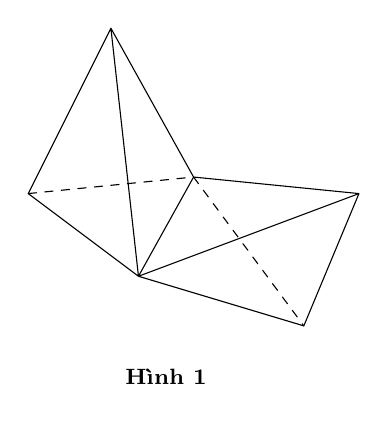
\begin{tikzpicture}[>=stealth,line join=round,line cap=round,font=\footnotesize,scale=.7]
			\path
			(0,0) coordinate (A)
			(3,0.3) coordinate (C)
			(1.5,3) coordinate (B)
			(2,-1.5) coordinate (D)
			(6,0) coordinate (E)
			(5,-2.4) coordinate (F);
			\draw (B)--(A)--(D)--(B)--(C)--(D)--(F)--(E)--(D) (C)--(E);
			\draw[dashed] (A)--(C)--(F);
			\path(2.5,-3)node[below]{\textbf{Hình 1}};
		\end{tikzpicture}\hspace{1cm}
		\begin{tikzpicture}[line join=round,line cap=round,line width=.6pt,font=\footnotesize,scale=.7]
			\path 
			(0,0) coordinate (A)
			(0,4) coordinate (A')
			(-20:2) coordinate (B)
			(20:3) coordinate (C)
			(60:3) coordinate (D)
			($(B)+(0,4)$) coordinate (B')
			($(C)+(0,4)$) coordinate (C')
			($(D)+(0,4)$) coordinate (D')
			;
			\draw (A)--(A')--(B')--(B)--(A) (A')--(C')--(C) (A')--(D') (1.88,0.68)--(C) (1.5,4.55)--(D');	
			\draw[dashed] (A)--(D) (A)--(1.88,0.68) (D)--(1.5,4.55);
			\path(1,-1)node[below]{\textbf{Hình 2}};
		\end{tikzpicture}\hspace{1cm}
		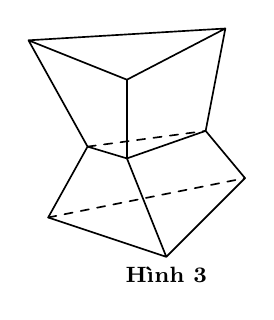
\begin{tikzpicture}[line join=round,line cap=round,line width=.6pt,font=\footnotesize,scale=.5]
			\path 
			(0,0) coordinate (A)
			(3,-1) coordinate (B)
			(5,1) coordinate (C)
			(1,1.8) coordinate (A')
			(2,1.5) coordinate (B')
			(4,2.2) coordinate (C')
			(-0.5,4.5) coordinate (A'')
			(2,3.5) coordinate (B'')
			(4.5,4.8) coordinate (C'')
			;
			\draw (A)--(B)--(C) (A')--(B')--(C') (A'')--(B'')--(C'')--(A'')--(A')--(A) (B'')--(B')--(B) (C'')--(C')--(C);
			\draw[dashed] (A)--(C) (A')--(C');
			\path (B) node[below]{\textbf{Hình 3}};
		\end{tikzpicture}\hspace{1cm}
		\begin{tikzpicture}[>=stealth,line join=round,line cap=round,font=\footnotesize,scale=.5]
			\path
			(0,0) coordinate (A)
			(4,0) coordinate (B)
			(-1.5,-2) coordinate (D)
			($(B)+(D)-(A)$) coordinate (C)
			($(A)+(0,4)$) coordinate (A')
			($(B)+(0,4)$) coordinate (B')
			($(C)+(0,4)$) coordinate (C')
			($(D)+(0,4)$) coordinate (D')
			(5,0.8) coordinate (E)
			(5.6,-1.2) coordinate (F)
			($(E)+(0,4)$) coordinate (E')
			($(F)+(0,4)$) coordinate (F');
			\draw (B')--(A')--(D')--(D)--(C)--(C')--(D') (C)--(B)--(F)--(F')--(E')--(B')--(C') (B)--(B')--(F');
			\draw[dashed] (A')--(A)--(D) (A)--(B)--(E)--(E') (E)--(F);
			\path (2,-2) node[below]{\textbf{Hình 4}};
		\end{tikzpicture}
	\end{center}
	\choice
	{Hình 4}
	{Hình 2}
	{Hình 1}
	{\True Hình 3}
	\loigiai{Hình 1, Hình 2, Hình 4 không phải hình đa diện vì nó vi phạm tính chất: `` mỗi cạnh là cạnh chung của đúng hai mặt''.}
\end{ex}
\begin{ex}%[2H1Y1-2]
	Cho đa giác đều $16$ đỉnh. Hỏi có bao nhiêu tam giác vuông có ba đỉnh là ba đỉnh của đa giác đều đó?
	\choice
	{$560$}
	{\True $112$}
	{$121$}
	{$128$}
	\loigiai{Ta có đa giác đều có $16$ đỉnh nên có $8$ đường chéo đi qua tâm. Ứng với mỗi đường chéo đi qua tâm có $14$ tam giác vuông. Vậy có $8\cdot 14=112$ tam giác.}
\end{ex}

\begin{ex}%[2H1Y2-3]
	Hình đa diện nào dưới đây \textbf{không} có tâm đối xứng?
	\choice
	{\True Tứ diện đều}
	{Bát diện đều}
	{Hình lập phương}
	{Lăng trụ lục giác đều}
	\loigiai{Dễ thấy tứ diện đều không có tâm đối xứng}
\end{ex}
	\begin{ex}%[2H1B2-3]
	Hình hộp chữ nhật có ba kích thước đôi một khác nhau có bao nhiêu mặt phẳng đối xứng?
	\choice
	{$6$ mặt phẳng}
	{$9$ mặt phẳng}
	{\True $3$ mặt phẳng}
	{$4$mặt phẳng}
	\loigiai
	{\immini{Xét hình hộp chữ nhật $ABCD.A'B'C'D'$ có ba kích thước đôi một khác nhau. \\
			Gọi $M, N, O, P, Q, R, S, T, X, U, V, W$ lần lượt là trung điểm của $AB, CD, C'D', A'B', AD, BC$, $B'C', A'D', DD', AA', BB', CC'$. 
			Khi đó có 3 mặt phẳng đối xứng là $\left(MNOP\right), \left(QRST\right), \left(XUVW\right)$}
		{\begin{tikzpicture}[>=stealth, line cap=round, line join=round,scale=0.6]
				\path
				(0,0) coordinate (A)
				(-135:3) coordinate (B)
				(0:8) coordinate (D)
				($(B)+(D)-(A)$) coordinate (C)
				(90:5) coordinate (A')
				($(A')+(B)-(A)$) coordinate (B')
				($(A')+(C)-(A)$) coordinate (C')
				($(A')+(D)-(A)$) coordinate (D');
				\coordinate (M) at ($(A)!0.5!(B)$);
				\coordinate (N) at ($(C)!0.5!(D)$);
				\coordinate (M') at ($(A')!0.5!(B')$);
				\coordinate (N') at ($(C')!0.5!(D')$);
				\coordinate (P) at ($(A)!0.5!(D)$);
				\coordinate (Q) at ($(C)!0.5!(B)$);
				\coordinate (P') at ($(A')!0.5!(D')$);
				\coordinate (Q') at ($(C')!0.5!(B')$);
				\coordinate (R) at ($(A)!0.5!(A')$);
				\coordinate (S) at ($(B)!0.5!(B')$);
				\coordinate (T) at ($(D)!0.5!(D')$);
				\coordinate (U) at ($(C)!0.5!(C')$);
				\draw[dashed] (A)--(B) (A)--(D) (A)--(A') (M)--(N) (M)--(M') (P)--(Q) (P)--(P') (R)--(T) (R)--(S);
				\draw (B)--(C)--(D)--(D')--(A')--(B')--(C')--(C) (B)--(B') (M')--(N')--(N) (P')--(Q')--(Q) (C')--(D')  (S)--(U)--(T); 
				\foreach \d/\g in{A/135,B/-90,C/-45,D/0,A'/135,B'/180,C'/0,D'/45}
				\draw[fill=black](\d)circle(1pt)node[shift={(\g:0.35)}]{$\d$};
	\end{tikzpicture}}}
\end{ex}
\begin{ex}%[2H1B2-3]
	Hình tứ diện đều có bao nhiêu trục đối xứng?
	\choice
	{$0$}
	{$1$}
	{\True $3$}
	{ $2$}
	\loigiai
	{Gọi $S$ là tập hợp các đỉnh của khối tứ diện đều $ABCD$. Giả sử $d$ là trục đối xứng của tứ diện đã cho, Phép đối xứng trục $d$ biến $S$ thành chính $S$ nên $d$ phải là trung trực của ít nhất một đoạn thẳng nối hai đỉnh bất kì của tứ diện.
		Vậy tứ diện đều có 3 trục đối xứng là các đường thẳng nối trung điểm của các cặp cạnh đối diện.}
\end{ex}
\begin{ex}%[2H1B2-3]
	Một hình hộp đứng có đáy là hình thoi (không phải là hình vuông) có bao nhiêu mặt phẳng đối xứng?
	\choice
	{$3$ mặt phẳng}
	{\True $4$ mặt phẳng}
	{ $2$ mặt phẳng}
	{ $1$ mặt phẳng}
	\loigiai
	{\immini{Hình hộp đứng có đáy là hình thoi có 3 mặt phẳng đối xứng trong đó bao gồm hai mặt phẳng chứa từng cặp đường chéo nhau song song của mỗi mặt đáy và 1 mặt phẳng cắt ngang tại trung điểm của chiều cao hình hộp. Cụ thể theo hình vẽ trên là $\left(BDEH\right), \left(ACGF\right), \left(IJKL\right)$}
		{\begin{tikzpicture}[>=stealth, line cap=round, line join=round,scale=0.6]
				\path
				(0,0) coordinate (A)
				(-135:3) coordinate (B)
				(0:8) coordinate (D)
				($(B)+(D)-(A)$) coordinate (C)
				(90:5) coordinate (A')
				($(A')+(B)-(A)$) coordinate (B')
				($(A')+(C)-(A)$) coordinate (C')
				($(A')+(D)-(A)$) coordinate (D');
				\coordinate (M) at ($(A)!0.5!(B)$);
				\coordinate (N) at ($(C)!0.5!(D)$);
				\coordinate (M') at ($(A')!0.5!(B')$);
				\coordinate (N') at ($(C')!0.5!(D')$);
				\coordinate (P) at ($(A)!0.5!(D)$);
				\coordinate (Q) at ($(C)!0.5!(B)$);
				\coordinate (P') at ($(A')!0.5!(D')$);
				\coordinate (Q') at ($(C')!0.5!(B')$);
				\coordinate (R) at ($(A)!0.5!(A')$);
				\coordinate (S) at ($(B)!0.5!(B')$);
				\coordinate (T) at ($(D)!0.5!(D')$);
				\coordinate (U) at ($(C)!0.5!(C')$);
				\draw[dashed] (A)--(B) (A)--(D) (A)--(A') (M)--(N) (M)--(M') (P)--(Q) (P)--(P') (R)--(T) (R)--(S);
				\draw (B)--(C)--(D)--(D')--(A')--(B')--(C')--(C) (B)--(B') (M')--(N')--(N) (P')--(Q')--(Q) (C')--(D')  (S)--(U)--(T); 
				\foreach \d/\g in{A/135,B/-90,C/-45,D/0,A'/135,B'/180,C'/0,D'/45}
				\draw[fill=black](\d)circle(1pt)node[shift={(\g:0.35)}]{$\d$};
	\end{tikzpicture}}}
\end{ex}
\begin{ex}%[2H1B2-3]
	Hình hộp chữ nhật có ba kích thước đôi một khác nhau có bao nhiêu mặt phẳng đối xứng?
	\choice
	{$6$ mặt phẳng}
	{$4$ mặt phẳng}
	{\True $3$ mặt phẳng}
	{ $9$ mặt phẳng}
	\loigiai
	{\immini{Xét hình hộp chữ nhật $ABCD.A'B'C'D'$ có ba kích thước đôi một khác nhau. \\
			Gọi $M, N, O, P, Q, R, S, T, X, U, V, W$ lần lượt là trung điểm của $AB, CD, C'D', A'B', AD, BC$, $B'C', A'D', DD', AA', BB', CC'$. 
			Khi đó có 3 mặt phẳng đối xứng là $\left(MNOP\right), \left(QRST\right), \left(XUVW\right)$}
		{\begin{tikzpicture}[>=stealth, line cap=round, line join=round,scale=0.6]
				\path
				(0,0) coordinate (A)
				(-135:3) coordinate (B)
				(0:8) coordinate (D)
				($(B)+(D)-(A)$) coordinate (C)
				(90:5) coordinate (A')
				($(A')+(B)-(A)$) coordinate (B')
				($(A')+(C)-(A)$) coordinate (C')
				($(A')+(D)-(A)$) coordinate (D');
				\coordinate (M) at ($(A)!0.5!(B)$);
				\coordinate (N) at ($(C)!0.5!(D)$);
				\coordinate (M') at ($(A')!0.5!(B')$);
				\coordinate (N') at ($(C')!0.5!(D')$);
				\coordinate (P) at ($(A)!0.5!(D)$);
				\coordinate (Q) at ($(C)!0.5!(B)$);
				\coordinate (P') at ($(A')!0.5!(D')$);
				\coordinate (Q') at ($(C')!0.5!(B')$);
				\coordinate (R) at ($(A)!0.5!(A')$);
				\coordinate (S) at ($(B)!0.5!(B')$);
				\coordinate (T) at ($(D)!0.5!(D')$);
				\coordinate (U) at ($(C)!0.5!(C')$);
				\draw[dashed] (A)--(B) (A)--(D) (A)--(A') (M)--(N) (M)--(M') (P)--(Q) (P)--(P') (R)--(T) (R)--(S);
				\draw (B)--(C)--(D)--(D')--(A')--(B')--(C')--(C) (B)--(B') (M')--(N')--(N) (P')--(Q')--(Q) (C')--(D')  (S)--(U)--(T); 
				\foreach \d/\g in{A/135,B/-90,C/-45,D/0,A'/135,B'/180,C'/0,D'/45}
				\draw[fill=black](\d)circle(1pt)node[shift={(\g:0.35)}]{$\d$};
	\end{tikzpicture}}}
\end{ex}
\begin{ex}%[2H1B2-3]
	Hình tứ diện đều có bao nhiêu mặt phẳng đối xứng?
	\choice
	{\True $6$}
	{$3$}
	{$4$}
	{ $2$}
	\loigiai
	{Hình tứ diện đều có 6 mặt phẳng đối xứng. \\
		\begin{center}
			\begin{tikzpicture}[scale=.4]
				\tkzDefPoints{0/0/A, 4/-2/B, 6/0/C}
				\coordinate (M) at ($(B)!.5!(C)$);
				\coordinate (H) at ($(A)!.67!(M)$);
				\coordinate (S) at ($(H)+(0,5)$);
				\coordinate (N) at ($(S)!.5!(C)$);
				\coordinate (P) at ($(B)!.5!(S)$);
				\coordinate (Q) at ($(S)!.5!(A)$);
				\coordinate (R) at ($(B)!.5!(A)$);
				\coordinate (K) at ($(A)!.5!(C)$);
				\draw[dashed] (M)--(A)--(C);
				\draw (B)--(A)--(S)--(M) (S)--(B)--(C)--(S);
				\fill[color=black!25, fill opacity=0.5] (S)--(M)--(A)--cycle;
			\end{tikzpicture}
			\begin{tikzpicture}[scale=.4]
				\tkzDefPoints{0/0/A, 4/-2/B, 6/0/C}
				\coordinate (M) at ($(B)!.5!(C)$);
				\coordinate (H) at ($(A)!.67!(M)$);
				\coordinate (S) at ($(H)+(0,5)$);
				\coordinate (N) at ($(S)!.5!(C)$);
				\coordinate (P) at ($(B)!.5!(S)$);
				\coordinate (Q) at ($(S)!.5!(A)$);
				\coordinate (R) at ($(B)!.5!(A)$);
				\coordinate (K) at ($(A)!.5!(C)$);
				\draw[dashed] (A)--(C);
				\draw (S)--(B)--(C)--(S)--(A)--(B) (A)--(P)--(C);
				\fill[color=black!25, fill opacity=0.5] (C)--(P)--(A)--cycle;
			\end{tikzpicture}
			\begin{tikzpicture}[scale=.4]
				\tkzDefPoints{0/0/A, 4/-2/B, 6/0/C}
				\coordinate (M) at ($(B)!.5!(C)$);
				\coordinate (H) at ($(A)!.67!(M)$);
				\coordinate (S) at ($(H)+(0,5)$);
				\coordinate (N) at ($(S)!.5!(C)$);
				\coordinate (P) at ($(B)!.5!(S)$);
				\coordinate (Q) at ($(S)!.5!(A)$);
				\coordinate (R) at ($(B)!.5!(A)$);
				\coordinate (K) at ($(A)!.5!(C)$);
				\draw[dashed] (A)--(C) (A)--(N);
				\draw (S)--(B)--(C)--(S)--(A)--(B)--(N);
				\fill[color=black!25, fill opacity=0.5] (A)--(B)--(N)--cycle;
			\end{tikzpicture}
			\begin{tikzpicture}[scale=.4]
				\tkzDefPoints{0/0/A, 4/-2/B, 6/0/C}
				\coordinate (M) at ($(B)!.5!(C)$);
				\coordinate (H) at ($(A)!.67!(M)$);
				\coordinate (S) at ($(H)+(0,5)$);
				\coordinate (N) at ($(S)!.5!(C)$);
				\coordinate (P) at ($(B)!.5!(S)$);
				\coordinate (Q) at ($(S)!.5!(A)$);
				\coordinate (R) at ($(B)!.5!(A)$);
				\coordinate (K) at ($(A)!.5!(C)$);
				\draw[dashed] (A)--(C) (S)--(K)--(B);
				\draw (S)--(B)--(C)--(S)--(A)--(B);
				\fill[color=black!25, fill opacity=0.5] (S)--(B)--(K)--cycle;
			\end{tikzpicture}
			\begin{tikzpicture}[scale=.4]
				\tkzDefPoints{0/0/A, 4/-2/B, 6/0/C}
				\coordinate (M) at ($(B)!.5!(C)$);
				\coordinate (H) at ($(A)!.67!(M)$);
				\coordinate (S) at ($(H)+(0,5)$);
				\coordinate (N) at ($(S)!.5!(C)$);
				\coordinate (P) at ($(B)!.5!(S)$);
				\coordinate (Q) at ($(S)!.5!(A)$);
				\coordinate (R) at ($(B)!.5!(A)$);
				\coordinate (K) at ($(A)!.5!(C)$);
				\draw[dashed] (A)--(C)--(R);
				\draw (S)--(B)--(C)--(S)--(A)--(B) (S)--(R);
				\fill[color=black!25, fill opacity=0.5] (S)--(R)--(C)--cycle;
			\end{tikzpicture}
			\begin{tikzpicture}[scale=.4]
				\tkzDefPoints{0/0/A, 4/-2/B, 6/0/C}
				\coordinate (M) at ($(B)!.5!(C)$);
				\coordinate (H) at ($(A)!.67!(M)$);
				\coordinate (S) at ($(H)+(0,5)$);
				\coordinate (N) at ($(S)!.5!(C)$);
				\coordinate (P) at ($(B)!.5!(S)$);
				\coordinate (Q) at ($(S)!.5!(A)$);
				\coordinate (R) at ($(B)!.5!(A)$);
				\coordinate (K) at ($(A)!.5!(C)$);
				\draw[dashed] (A)--(Q)--(C)--(A);
				\draw (S)--(B)--(C)--(S)--(A)--(B)--(Q);
				\fill[color=black!25, fill opacity=0.5] (B)--(Q)--(C)--cycle;
			\end{tikzpicture}
	\end{center}}
\end{ex}
\begin{ex}%[2H1B2-3]
	Hình nào sau đây không có trục đối xứng?
	\choice
	{\True Hình hộp xiên}
	{Tam giác đều}
	{Hình tròn}
	{Đường thẳng}
	\loigiai
	{Đường tròn có vô số trục đối xứng.
		Đường thẳng có một trục đối xứng trùng với nó.
		Tam giác đều có 3 trục đối xứng, các trục này đi qua trọng tâm của tam giác đều.
		Hình hộp xiên không có trục đối xứng}
\end{ex}
\begin{ex}%[2H1B2-3]
	Biết rằng một hình đa diện $H$ có 6 mặt là 6 tam giác đều. Hãy chỉ ra mệnh đề nào dưới đây là đúng?
	\choice
	{ Không tồn tại hình $H$ nào có mặt phẳng đối xứng}
	{\True Có tồn tại một hình $H$ có 4 mặt phẳng đối xứng}
	{Không tồn tại hình $H$ nào có đúng 5 đỉnh}
	{Có tồn tại hình $H$ có hai tâm đối xứng phân biệt}
	\loigiai
	{Luôn tồn tại hình đa diện $H$ có mặt phẳng đối xứng và có đúng $5$ đỉnh, $H$ không có tâm đối xứng}
\end{ex}
\begin{ex}%[2H1Y2-3]%Câu 38[2H1Y2-3]
	[Chuyên Thái Bình-2018] Hình chóp tứ giác đều có bao nhiêu mặt phẳng đối xứng?
	\choice
	{$2$}
	{$6$}
	{$8$}
	{\True $4$}
	\loigiai{
		\immini{Đó là các mặt phẳng $\left(SAC\right)$ , $\left(SBD\right)$ , $\left(SEF\right)$ , $\,\left(SMN\right)$ với $E$ , $M$ , $F$ , $N$ là các trung điểm của các cạnh $AB,$ $CB,$ $CD,$ $AD$ (hình vẽ bên).}
		{\begin{tikzpicture}[line join=round, line cap=round,thick,scale=0.6]
				\coordinate (A) at (0,0);
				\coordinate (B) at (-3,-2);
				\coordinate (D) at (6,0);
				\coordinate (C) at ($(B)+(D)-(A)$);
				\coordinate (O) at ($(A)!0.5!(C)$);
				\coordinate (S) at ($(O)+(0,5)$);
				\coordinate (G) at ($(A)!0.5!(B)$);
				\coordinate (H) at ($(C)!0.5!(B)$);
				\coordinate (I) at ($(C)!0.5!(D)$);
				\coordinate (J) at ($(A)!0.5!(D)$);
				\draw(S)--(D) (S)--(B) (S)--(C)  (B)--(C)(C)--(D) (S)--(H) (S)--(I);
				\draw[dashed,thin](A)--(C) (A)--(D) (A)--(B) (S)--(A) (S)--(O) (B)--(D) (S)--(G)(S)--(J) (G)--(I) (H)--(J);
				\pic[draw,thin,angle radius=2mm] {right angle = S--O--D} pic[draw,thin,angle radius=2mm] {right angle = S--O--A};
				\foreach \i/\g in {S/90,A/180,B/-90,C/-90,D/0,O/-90,G/180,H/-90,I/0,J/90}{\draw[fill=white](\i) circle (1.5pt) ($(\i)+(\g:3mm)$) node[scale=1]{$\i$};}
		\end{tikzpicture}}
	}
\end{ex}
%Câu 39
\begin{ex}%[2H1Y2-3]
	[Chuyên Quốc Học Huế-2018] Hình đa diện nào dưới đây không có tâm đối xứng?
	\choice
	{Hình bát diện đều}
	{Hình tứ diện đều}
	{Hình lập phương}
	{\True Hình lăng trụ tứ giác đều}
	\loigiai
	{Ta có phép đối xứng tâm $I$ biến hình $(H)$ thành chính nó. Khi đó hình $(H)$ có tâm đối xứng là $I$ suy ra hình lăng trụ tứ giác đều, hình bát diện đều và hình lập phương là các hình đa diện có tâm đối xứng.}
\end{ex}

\begin{ex}%Câu 40%[2H1Y2-3]
	[Chuyên Hạ Long-QNinh-2018] Hình nào dưới nào dưới đây không có trục đối xứng?
	\choice
	{Tam giác cân}
	{Hình thang cân}
	{Hình elip}
	{\True Hình bình hành}
	\loigiai
	{
	}
\end{ex}

\begin{ex}%Câu 41%[2H1Y2-3]
	[THPT Đặng Thúc Hứa-Nghệ An-2018] Hình lăng trụ tam giác đều có tất cả các cạnh bằng nhau có bao nhiêu mặt phẳng đối xứng?
	\choice
	{\True $ 4$}
	{$ 3$}
	{$ 5$}
	{$ 6$}
	\loigiai{
		Có $ 4$ mặt phẳng đối xứng như hình vẽ sau.\\
		\begin{center}
			\begin{tikzpicture}[line join=round, line cap=round,thick,scale=0.8]
				\coordinate (A') at (0,4);
				\coordinate (A) at (0,0);
				\coordinate (B) at (3,-2);
				\coordinate (C) at (4,0);
				\coordinate (C') at ($(C)+(0,4)$);
				\coordinate (B') at ($(B)+(0,4)$);
				\coordinate (M) at ($(B)!0.5!(C)$);
				\coordinate (M') at ($(B')!0.5!(C')$);
				\draw(A)--(B) (B')--(A')--(C')--(B')--(B)--(C)--(C') (A)--(A') (A')--(M')--(M);
				\draw[dashed,thin](A)--(C) (A)--(M);
				\fill[pattern=grid](A)--(M)--(M')--(A')--cycle;
				%\foreach \i/\g in {S/90,A/180,B/-90,C/0}{\draw[fill=white](\i) circle (1.5pt) ($(\i)+(\g:3mm)$) node[scale=1]{$\i$};}
			\end{tikzpicture}\hspace{1cm}				\begin{tikzpicture}[line join=round, line cap=round,thick,scale=0.8]
				\coordinate (A') at (0,4);
				\coordinate (A) at (0,0);
				\coordinate (B) at (3,-2);
				\coordinate (C) at (4,0);
				\coordinate (C') at ($(C)+(0,4)$);
				\coordinate (B') at ($(B)+(0,4)$);
				\coordinate (M) at ($(B)!0.5!(A)$);
				\coordinate (M') at ($(B')!0.5!(A')$);
				\draw(A)--(B) (B')--(A')--(C')--(B')--(B)--(C)--(C') (A)--(A') (C')--(M')--(M);
				\draw[dashed,thin](A)--(C) (C)--(M);
				\fill[pattern=grid](C)--(M)--(M')--(C')--cycle;
				%\foreach \i/\g in {S/90,A/180,B/-90,C/0}{\draw[fill=white](\i) circle (1.5pt) ($(\i)+(\g:3mm)$) node[scale=1]{$\i$};}
			\end{tikzpicture}\hspace{1cm}
			\begin{tikzpicture}[line join=round, line cap=round,thick,scale=0.8]
				\coordinate (A') at (0,4);
				\coordinate (A) at (0,0);
				\coordinate (B) at (3,-2);
				\coordinate (C) at (4,0);
				\coordinate (C') at ($(C)+(0,4)$);
				\coordinate (B') at ($(B)+(0,4)$);
				\coordinate (M) at ($(A)!0.5!(C)$);
				\coordinate (M') at ($(A')!0.5!(C')$);
				\draw(A)--(B) (B')--(A')--(C')--(B')--(B)--(C)--(C') (A)--(A') (B')--(M');
				\draw[dashed,thin](A)--(C) (B)--(M)--(M');
				\fill[pattern=grid](B)--(M)--(M')--(B')--cycle;
				%\foreach \i/\g in {S/90,A/180,B/-90,C/0}{\draw[fill=white](\i) circle (1.5pt) ($(\i)+(\g:3mm)$) node[scale=1]{$\i$};}
			\end{tikzpicture}\hspace{1cm}
			\begin{tikzpicture}[line join=round, line cap=round,thick,scale=0.8]
				\coordinate (A') at (0,4);
				\coordinate (A) at (0,0);
				\coordinate (B) at (3,-2);
				\coordinate (C) at (4,0);
				\coordinate (C') at ($(C)+(0,4)$);
				\coordinate (B') at ($(B)+(0,4)$);
				\coordinate (M) at ($(A)!0.5!(A')$);
				\coordinate (N) at ($(B')!0.5!(B)$);
				\coordinate (P) at ($(C')!0.5!(C)$);
				\draw(A)--(B) (B')--(A')--(C')--(B')--(B)--(C)--(C') (A)--(A') (M)--(N)--(P);
				\draw[dashed,thin](A)--(C) (M)--(P);
				\fill[pattern=grid](M)--(N)--(P)--cycle;
				%\foreach \i/\g in {S/90,A/180,B/-90,C/0}{\draw[fill=white](\i) circle (1.5pt) ($(\i)+(\g:3mm)$) node[scale=1]{$\i$};}
			\end{tikzpicture}
		\end{center}
	}
\end{ex}
\begin{ex}%Câu 42%[2H1Y2-3]
	[Vĩnh Phúc-2018] Khối bát diện đều có bao nhiêu mặt phẳng đối xứng?
	\choice
	{$ 8$}
	{$ 4$}
	{\True $ 9$}
	{$ 6$}
	\loigiai{\immini{Hình bát diện $ABCDEF$ có $9$ mặt phẳng đối xứng gồm $3$ mặt phẳng $(ABCD), (AECF), (BEDF)$ và $6$ mặt phẳng mà mỗi mặt phẳng là mặt phẳng trung trực của hai cạnh song song.}{\begin{tikzpicture}[line join=round, line cap=round,thick,scale=0.5]
				\coordinate (A) at (0,0);
				\coordinate (B) at (2,-2);
				\coordinate (D) at (5,0);
				\coordinate (C) at ($(B)+(D)-(A)$);
				\coordinate (O) at ($(A)!0.5!(C)$);
				\coordinate (E) at ($(O)+(0,6)$);
				\coordinate (F) at ($(O)!-1!(E)$);
				\draw(E)--(A) (E)--(B) (E)--(C) (A)--(B) (B)--(C)--(F)--(B) (F)--(A) ;
				\draw[dashed,thin](A)--(C) (A)--(D) (C)--(D) (E)--(D) (E)--(O) (B)--(D)--(F)--(O);
				\pic[draw,thin,angle radius=2mm] {right angle = E--O--D} pic[draw,thin,angle radius=2mm] {right angle = E--O--A};
				\foreach \i/\g in {E/90,A/180,B/180,C/-90,D/0,O/-90,F/-90}{\draw[fill=white](\i) circle (1.5pt) ($(\i)+(\g:3mm)$) node[scale=1]{$\i$};}
		\end{tikzpicture}}
	}
\end{ex}

\begin{ex}%Câu 43%[2H1Y1-4]
	[Trần Phú-Hải Phòng-2019]
	Cho khối lập phương $ABCD.A'B'C'D'$. Phép đối xứng qua mặt phẳng $(ABC'D')$ biến khối tứ diện $BCDD'$ thành khối tứ diện nào sau đây?
	\choice
	{$BCA'D'$}
	{\True $BB'A'D'$}
	{$B'BC'A'$}
	{$BC'D'A'$}
	\loigiai
	{\immini{Ký hiệu $\text{Đ}$ là phép đối xứng qua mặt phẳng $(ABC'D')$.\\
			Ta có $\text{Đ}(B)=B$, $\text{Đ}(C)=B'$,
			$\text{Đ}(D)=A'$, $\text{Đ}(D')=D'$.\\
			Vậy phép đối xứng qua mặt phẳng $ABC'D'$ biến khối tứ diện $BCDD'$ thành khối tứ diện $BB'A'D'$.
		}{\begin{tikzpicture}[line join=round, line cap=round,thick,scale=0.8]
				\coordinate (A') at (0,4);
				\coordinate (A) at (0,0);
				\coordinate (C) at (3,-2);
				\coordinate (D) at (4,0);
				\coordinate (B) at ($(A)+(-1,-2)$);
				\coordinate (D') at ($(D)+(0,4)$);
				\coordinate (C') at ($(C)+(0,4)$);
				\coordinate (B') at ($(B)+(0,4)$);
				\draw(A')--(B')-- (C')--(D')--(A') (B)--(C)--(D)--(D') (B)--(B')(C)--(C')(B)--(C') ;
				\draw[dashed,thin](A)--(B) (A)--(D) (A)--(A') (A)--(D');
				\foreach \i/\g in {A'/90,A/180,B/-90,C/0,D/0,B'/180,C'/0,D'/0}{\draw[fill=white](\i) circle (1.5pt) ($(\i)+(\g:3mm)$) node[scale=1]{$\i$};}
		\end{tikzpicture}}		
	}
\end{ex}	
%Câu 44
\begin{ex}[Mã 110 - 2017]%[2H1Y1-3]
	Mặt phẳng $(AB'C')$ chia khối lăng trụ $ABC.A'B'C'$ thành các khối đa diện nào?
	\choice
	{Hai khối chóp tam giác}
	{Hai khối chóp tứ giác}
	{\True Một khối chóp tam giác và một khối chóp tứ giác}
	{Một khối chóp tam giác và một khối chóp ngũ giác}
	\loigiai{
		\immini{
			Mặt phẳng $(AB'C')$ chia khối lăng trụ $ABC.A'B'C'$ thành một khối chóp tam giác $A.A'B'C'$ và một khối chóp tứ giác $A.BB'C'C$.
		}{\begin{tikzpicture}[line join=round, line cap=round,thick,scale=0.8]
				\coordinate (A') at (0,4);
				\coordinate (A) at (0,0);
				\coordinate (B) at (3,-2);
				\coordinate (C) at (4,0);
				\coordinate (C') at ($(C)+(0,4)$);
				\coordinate (B') at ($(B)+(0,4)$);
				\draw(A)--(B) (B')--(A')--(C')--(B')--(B)--(C)--(C') (A)--(A') (A)--(B');
				\draw[dashed,thin](A)--(C) (A)--(C');
				\foreach \i/\g in {C'/0,B'/0,A'/180,A/180,B/-90,C/0}{\draw[fill=white](\i) circle (1.5pt) ($(\i)+(\g:3mm)$) node[scale=1]{$\i$};}
			\end{tikzpicture}
		}
	}
\end{ex}
\begin{ex}%[2H1B1-3]
	[THPT An Lão Hải Phòng 2019] Cắt khối trụ $ ABC{.}A'B'C'$ bởi các mặt phẳng $\left(AB'C'\right)$ và $\left(ABC'\right)$ ta được những khối đa diện nào?
	\choice
	{Hai khối tứ diện và hai khối chóp tứ giác}
	{\True Ba khối tứ diện}
	{Một khối tứ diện và hai khối chóp tứ giác}
	{Hai khối tứ diện và một khối chóp tứ giác}
	\loigiai{
		
		\immini{
			Ba khối tứ diện là $A{.}A'B'C'$, $A{.}BB'C'$, $A{.}BCC'$.
		}{
			\begin{tikzpicture}[scale=.7]
				\tikzset{every node/.style={scale=0.7}}%
				\coordinate (A) at (1.3,-1);
				\coordinate (C) at (0,0);
				\coordinate (B) at (5,0);
				\coordinate (z) at (1,4.5);
				\coordinate (A) at (1.3,-1);
				\coordinate (C') at ($(C)+(z)$);
				\coordinate (B') at ($(B)+(z)$);
				\coordinate (A') at ($(A)+(z)$);
				\draw (A')--(B')--(C')--(A')--(A)--(B)--(B') (C)--(A)--(C')--(C) (A)--(B');
				%	\tkzDrawSegments(D,A A,B B,C B,E C,F D,E E,F F,D)
				\draw[dashed] (C)--(B)--(C') ;
				%		%	\draw ([yshift=-0.15cm]E) -- ([yshift=-0.15cm]F) node[midway, below]{6 cm};
				%		\draw pic[draw,angle radius=2mm] {right angle = F--E--G};
				\draw[fill=black] (A) node[below]{$A$} circle (1pt)  
				(B) circle (1pt) node[below]{$B$} 
				(C) circle (1pt) node[below]{$C$} 
				(A') circle (1pt) node[above]{$A'$}		 
				(B') circle (1pt) node[above]{$B'$}
				(C') circle (1pt) node[above]{$C'$};
			\end{tikzpicture}
		}
	}
\end{ex}

\begin{ex}%[2H1B1-3]
	[THPT Đoàn Thượng-Hải Phòng-2018] Cho khối tứ diện $ ABCD$. Lấy điểm $ M$ nằm giữa $ A$ và $ B$, điểm $ N$ nằm giữa $ C$ và $ D$. Bằng hai mặt phẳng $\left(CDM\right)$ và $\left(ABN\right)$, ta chia khối tứ diện đó thành bốn khối tứ diện nào sau đây?
	\choice
	{$ NACB$, $ BCMN$, $ ABND$, $ MBND$}
	{$ MANC$, $ BCDN$, $ AMND$, $ ABND$}
	{\True $ MANC$, $ BCMN$, $ AMND$, $ MBND$}
	{$ ABCN$, $ ABND$, $ AMND$, $ MBND$}
	\loigiai
	{
		\immini{	Bằng hai mặt phẳng $\left(CDM\right)$ và $\left(ABN\right)$, ta chia khối tứ diện đó thành bốn khối tứ diện:\\
			$ MANC$, $ BCMN$, $ AMND$, $ MBND$.}{
			
			\begin{tikzpicture}[scale=.7]
				\tikzset{every node/.style={scale=0.7}}%
				\coordinate (A) at (1.3,4);
				\coordinate (B) at (0,0);
				\coordinate (D) at (5,0);
				\coordinate (C) at (2,-1);
				\coordinate (M) at ($(B)!0.4!(A)$);
				\coordinate (N) at ($(C)!0.6!(D)$);
				\draw (N)--(A)--(B)--(C)--(D)--(A)--(C)--(M) ;
				\draw[dashed] (D)--(B)--(N)--(M)--(D);
				%		%	\draw ([yshift=-0.15cm]E) -- ([yshift=-0.15cm]F) node[midway, below]{6 cm};
				%		\draw pic[draw,angle radius=2mm] {right angle = F--E--G};
				\draw[fill=black] (A) node[above]{$A$} circle (1pt)  
				(B) circle (1pt) node[left]{$B$} 
				(C) circle (1pt) node[below]{$C$} 
				(D) circle (1pt) node[right]{$D$}		 
				(M) circle (1pt) node[above left]{$M$}
				(N) circle (1pt) node[below right]{$N$};
			\end{tikzpicture}
		}
		
	}
\end{ex}

\begin{ex}%[2H1B1-3]
	[THPT An Lão 2017] Cắt khối trụ $ ABC{.}A'B'C'$ bởi các mặt phẳng $\left(AB'C'\right)$ và $\left(ABC'\right)$ ta được những khối đa diện nào?
	\choice
	{Một khối tứ diện và hai khối chóp tứ giác}
	{\True Ba khối tứ diện}
	{Hai khối tứ diện và hai khối chóp tứ giác}
	{Hai khối tứ diện và một khối chóp tứ giác}
	\loigiai{
		\immini{		
			Ta có ba khối tứ diện là $ A{.}A'B'C'$; $B'{.}ABC'$; $C'{.}ABC$.}{
			\begin{tikzpicture}[scale=.7]
				\tikzset{every node/.style={scale=0.7}}%
				\coordinate (A) at (1.3,-1);
				\coordinate (C) at (0,0);
				\coordinate (B) at (5,0);
				\coordinate (z) at (1,4.5);
				\coordinate (A) at (1.3,-1);
				\coordinate (C') at ($(C)+(z)$);
				\coordinate (B') at ($(B)+(z)$);
				\coordinate (A') at ($(A)+(z)$);
				\draw (A')--(B')--(C')--(A')--(A)--(B)--(B') (C)--(A)--(C')--(C) (A)--(B');
				%	\tkzDrawSegments(D,A A,B B,C B,E C,F D,E E,F F,D)
				\draw[dashed] (C)--(B)--(C') ;
				%		%	\draw ([yshift=-0.15cm]E) -- ([yshift=-0.15cm]F) node[midway, below]{6 cm};
				%		\draw pic[draw,angle radius=2mm] {right angle = F--E--G};
				\draw[fill=black] (A) node[below]{$A$} circle (1pt)  
				(B) circle (1pt) node[below]{$B$} 
				(C) circle (1pt) node[below]{$C$} 
				(A') circle (1pt) node[above]{$A'$}		 
				(B') circle (1pt) node[above]{$B'$}
				(C') circle (1pt) node[above]{$C'$};
			\end{tikzpicture}
		}
		
	}	
\end{ex}

\begin{ex}%[2H1B1-3]
	[THPT Ngô Quyền-2017] Cắt khối lăng trụ $MNP{.}M'N'P'$ bởi các mặt phẳng $\left(MN'P'\right)$ và $\left(MNP'\right)$ ta được những khối đa diện nào?
	\choice
	{\True Ba khối tứ diện}
	{Hai khối tứ diện và một khối chóp tứ giác}
	{Hai khối tứ diện và hai khối chóp tứ giác}
	{Một khối tứ diện và một khối chóp tứ giác}
	\loigiai{
		\immini{	
			Cắt khối lăng trụ $MNP{.}M'N'P'$ bởi các mặt phẳng $\left(MN'P'\right)$ và $\left(MNP'\right)$ ta được ba khối tứ diện là $P{.}MNP'$; $P{.}MNN'$; $M'{.}MN'P'$.}{
			\begin{tikzpicture}[scale=.7]
				\tikzset{every node/.style={scale=0.7}}%
				\coordinate (A) at (1.3,-1);
				\coordinate (C) at (0,0);
				\coordinate (B) at (5,0);
				\coordinate (z) at (1,4.5);
				\coordinate (A) at (1.3,-1);
				\coordinate (C') at ($(C)+(z)$);
				\coordinate (B') at ($(B)+(z)$);
				\coordinate (A') at ($(A)+(z)$);
				\draw (A')--(B')--(C')--(A')--(A)--(B)--(B') (C)--(A)--(C')--(C) (A)--(B');
				%	\tkzDrawSegments(D,A A,B B,C B,E C,F D,E E,F F,D)
				\draw[dashed] (C)--(B)--(C') ;
				%		%	\draw ([yshift=-0.15cm]E) -- ([yshift=-0.15cm]F) node[midway, below]{6 cm};
				%		\draw pic[draw,angle radius=2mm] {right angle = F--E--G};
				\draw[fill=black] (A) node[below]{$P'$} circle (1pt)  
				(B) circle (1pt) node[below]{$N'$} 
				(C) circle (1pt) node[below]{$M'$} 
				(A') circle (1pt) node[above]{$P$}		 
				(B') circle (1pt) node[above]{$N$}
				(C') circle (1pt) node[above]{$M$};
			\end{tikzpicture}	
			
		}
		
	}
	
\end{ex}

\begin{ex}%[2H1K1-3]
	[THPT Yên Định-Thanh Hóa 2018] Có thể chia một khối lập phương thành bao nhiêu khối tứ diện có thể tích bằng nhau mà các đỉnh của tứ diện cũng là đỉnh của hình lập phương?
	\choice
	{$2$}
	{$8$}
	{$4$}
	{\True $6$}
	\loigiai{
		\immini{
			\begin{itemize}
				\item	Ta chia khối lập phương thành hai khối lăng trụ đứng.
				\item Ứng với mỗi khối lăng trụ đứng ta có thể chia thành ba khối tứ diện mà các đỉnh của tứ diện cũng là đỉnh của hình lập phương.
			\end{itemize}
			
			Vậy có tất cả là $6$ khối tứ diện có thể tích bằng nhau.}{
			\begin{tikzpicture}[scale=.7]
				\tikzset{every node/.style={scale=0.7}}%
				\coordinate (B) at (0,0);
				\coordinate (C) at (5,0);
				\coordinate (A) at (-2,-1.5);
				\coordinate (D) at ($(C)+(A)$);
				\coordinate (z) at (0,-5);
				\coordinate (A') at ($(A)+(z)$);
				\coordinate (B') at ($(B)+(z)$);
				\coordinate (C') at ($(C)+(z)$);
				\coordinate (D') at ($(D)+(z)$);
				\draw (A)--(B)--(C)--(D)--(A)--(A')--(D')--(C')--(C) (C')--(D)--(D')--(A) (B)--(D);
				\draw[dashed] (B)--(B')--(A') (A)--(B')--(D') (B)--(C')--(B')--(D);
				%		%	\draw ([yshift=-0.15cm]E) -- ([yshift=-0.15cm]F) node[midway, below]{6 cm};
				%		\draw pic[draw,angle radius=2mm] {right angle = F--E--G};
				\draw[fill=black] (A) node[above]{$A$} circle (1pt)  
				(B) circle (1pt) node[above]{$B$} 
				(C) circle (1pt) node[above]{$C$} 
				(D) circle (1pt) node[above]{$D$} 
				(A') circle (1pt) node[below]{$A'$}		 
				(B') circle (1pt) node[below]{$B'$}
				(C') circle (1pt) node[below]{$C'$}
				(D') circle (1pt) node[below]{$D'$};
			\end{tikzpicture}	
			
		}
		
	}
\end{ex}

\begin{ex}%[2H1K1-2]
	[THPT Lương Thế Vinh Hà Nội 2019] Cho đa giác đều có $ 2018$ đỉnh. Hỏi có bao nhiêu hình chữ nhật có $ 4$ đỉnh là các đỉnh của đa giác đã cho?
	\choice
	{$ \mathrm{C}_{2018}^4$}
	{$ \mathrm{C}_{1009}^4$}
	{$ \mathrm{C}_{2018}^2$}
	{\True $ \mathrm{C}_{1009}^2$}
	\loigiai{
		Số đường chéo đi qua tâm của đa giác đều $ 2018$ đỉnh là  $ 1009$.\\
		Cứ hai đường chéo đi qua tâm tạo thành một hình chữ nhật. Vậy số hình chữ nhật có $ 4$ đỉnh là các đỉnh của đa giác đã cho là $ \mathrm{C}_{1009}^2$.\\
	}
\end{ex}
\Closesolutionfile{ans}
\indapan{10}{ans/CD9/Muc_5_6}

